% ===========================================================================
% Article A (scientific): Group-theoretic discrimination of twin operation spaces
% Narrative arc: antecedents -> general theory -> generalization -> applications
% ===========================================================================
\documentclass[11pt,a4paper]{article}
\usepackage[utf8]{inputenc}
\usepackage[T1]{fontenc}
\usepackage{lmodern}
\usepackage[english]{babel}
\usepackage{amsmath,amssymb,amsthm,amsfonts}
\usepackage{booktabs}
\usepackage{graphicx}
\usepackage[margin=1in]{geometry}
\usepackage{xcolor}
\usepackage{hyperref}
\hypersetup{colorlinks=true, linkcolor=blue!60!black, citecolor=blue!50!black,
            urlcolor=blue!60!black}

\newcommand{\Op}{\mathrm{Op}}
\newcommand{\Z}{\mathbb{Z}}
\newcommand{\R}{\mathbb{R}}
\newcommand{\C}{\mathbb{C}}
\newcommand{\Norm}{\mathrm{N}}
\newcommand{\code}[1]{\texttt{#1}}

\theoremstyle{plain}
\newtheorem{theorem}{Theorem}
\newtheorem{proposition}[theorem]{Proposition}
\newtheorem{corollary}[theorem]{Corollary}
\theoremstyle{definition}
\newtheorem{definition}[theorem]{Definition}
\theoremstyle{remark}
\newtheorem{remark}[theorem]{Remark}

\title{\textbf{Group-Theoretic Discrimination of Twin Operation Spaces}\\[0.3em]
\large From Non-Newtonian Calculus to the Class Equation and Weyl Integration}
\author{Jocelyn Nemb\'e\\
\small Modeling and Calculus Laboratory, National Institute of Management
Sciences, Libreville, Gabon\\
\small ROOTS-INSIGHTS \quad\textbar\quad \texttt{jnembe@roots-insights.org}}
\date{June 2026}

\begin{document}
\maketitle

\begin{abstract}
\noindent
Generator-function arithmetics --- non-Newtonian calculus, the multiplicative
and bigeometric calculi, and the exponential hierarchy of operations --- are
classically presented as isolated constructions
$x\oplus_\varphi y=\varphi^{-1}(\varphi(x)+\varphi(y))$. We place them in a
single general theory: each is the \emph{twin operation}
$x\odot_{eg}y=g^{-1}\!\cdot\!\bigl((g\cdot x)\odot_e(g\cdot y)\bigr)$ for a
monogenic group $G=\langle\varphi\rangle$, an instance of the operation space
$\Op(E,\odot_e;G)$. We then \emph{generalize} from monogenic $\Z$ to arbitrary
symmetry groups and develop the invariants that \emph{discriminate} among the
resulting operations: the class equation for finite groups, primary
decomposition for abelian groups, and Weyl integration for compact Lie groups.
Along the way we correct the classification theorem of the literature: $\Op$ is
the homogeneous space $G/L$, a group \emph{iff} the structural kernel $L$ is
normal (computed counterexample: $S_4$ on $+\bmod 4$). Finally we apply the
generalizations and compare with the existing record: the discrimination of
operation spaces into decision cells, the Weyl measure verified against
random-matrix (CUE) statistics and Schur-character orthonormality, and the
classical magma counts ($n^n$, $q^{q+3}$, $S_n\!\to\!2$) recovered as special
cases. Each statement is reproducible; the library carries $131$ passing tests.
\end{abstract}

\noindent\textbf{Keywords:} non-Newtonian calculus, transport of structure,
classification $G/L$, class equation, Weyl integration, Schur characters.\\
\textbf{MSC 2020:} 20B25, 20C30, 22E46, 26A24, 65--04.

\section{Introduction}

This paper follows a deliberate arc. We (1) recall the prior constructions of
deformed arithmetic and what they contributed; (2) show that they all sit inside
one general theory of \emph{transport of structure}; (3) generalize that theory
from cyclic to arbitrary symmetry groups; and (4) apply the generalization ---
discriminating operation spaces by group-theoretic invariants --- comparing the
outcomes with the existing record. The viewpoint is scientific and
computational: every claim is matched to a reproducible calculation.

\section{Antecedents and their contributions}
\label{sec:prior}

\paragraph{Non-Newtonian and multiplicative calculus.}
Grossman and Katz \cite{grossman} replaced the additive pair $(+,\cdot)$ by
operations built from a generator $\varphi$,
\begin{equation}\label{eq:nn}
x\oplus_\varphi y=\varphi^{-1}\bigl(\varphi(x)+\varphi(y)\bigr),\qquad
x\otimes_\varphi y=\varphi^{-1}\bigl(\varphi(x)\cdot\varphi(y)\bigr),
\end{equation}
yielding the multiplicative ($\varphi=\log$) and bigeometric calculi. Their
contribution was a working family of calculi --- derivatives, integrals, means
--- adapted to multiplicative phenomena, and the recognition that the ``shape''
of arithmetic is a modelling choice.

\paragraph{Transport of structure and deformation.}
In algebra, conjugating an operation by a map, $a\diamond_g b=g^{-1}(g(a)\diamond
g(b))$, is the canonical equivariant deformation; its orbit theory is governed
by the orbit--stabilizer and first-isomorphism theorems, and its obstructions by
Gerstenhaber--Hochschild deformation cohomology \cite{gerstenhaber}. This
supplied the structural language but was rarely applied to \emph{operations} as
the deformed objects.

\paragraph{The exponential hierarchy.}
A recent foundations volume organizes \eqref{eq:nn} for $\varphi=\exp$ into a
chain $+\to\cdot\to x^{\ln y}\to\cdots$, the level-$n$ operation being
$\exp^{(-n)}(\exp^{(n)}x+\exp^{(n)}y)$, and proposes a classification of the
induced operations. Its contribution was to expose an infinite ladder of
coherent arithmetics; its classification, however, over-claims a group
structure, which we correct below.

\paragraph{Spectral side.}
On the eigenvalue side, Weyl's integration formula and the random-matrix theory
of the classical compact groups \cite{weyl,mehta,mezzadri} describe the
distribution of conjugacy classes; these will provide both the tool and the
benchmark for the Lie-group generalization.

\section{The general theory and its corrected classification}
\label{sec:theory}

\begin{definition}[Transport]
Let a group $G$ act on a set $E$ with a binary operation $\odot_e$. The
\emph{twin operation} of $g\in G$ is
\begin{equation}\label{eq:transport}
x\odot_{eg}y:=g^{-1}\cdot\bigl((g\cdot x)\odot_e(g\cdot y)\bigr).
\end{equation}
Write $\pi:G\to\Op(E,\odot_e;G)$, $g\mapsto\odot_{eg}$, and let
$L=\{g:\odot_{eg}=\odot_e\}$ be the \emph{structural kernel}.
\end{definition}

Every antecedent of \S\ref{sec:prior} is the special case
$G=\langle\varphi\rangle$ monogenic: \eqref{eq:nn} is \eqref{eq:transport} for
the action $n\cdot x=\varphi^{(n)}(x)$, and the exponential hierarchy is
$G=\langle\exp\rangle\cong\Z$. Thus non-Newtonian calculus and the hierarchy are
\emph{points} of a single object $\Op$.

\begin{proposition}[Kernel and fibres]\label{prop:fibres}
$L$ is a subgroup of $G$, and
$\odot_{eg}=\odot_{eh}\iff hg^{-1}\in L\iff Lg=Lh$.
\end{proposition}

\begin{proof}
Equality of \eqref{eq:transport} for $g,h$, after applying $h\cdot(-)$ and
substituting $u=g\cdot x,\ v=g\cdot y$, reads $m\cdot(u\odot_e v)=(m\cdot
u)\odot_e(m\cdot v)$ with $m=hg^{-1}$, i.e. $m\in L$.
\end{proof}

\begin{corollary}[Classification]\label{cor:class}
$Lg\mapsto\odot_{eg}$ is a bijection $L\backslash G\to\Op$; hence
$|\Op|=[G:L]$ and $\Op$ is a homogeneous $G$-set.
\end{corollary}

\begin{remark}[What it means]
The operation space is not free data: it is rigidly the coset space
$L\backslash G$, so its size and structure are fixed by the pair $(G,L)$ alone.
Choosing a twin operation is choosing a coset --- nothing more, nothing less.
\end{remark}

\begin{theorem}[Group structure $\iff$ normality]\label{thm:normal}
$\odot_{eg}\ast\odot_{eh}:=\odot_{e,gh}$ is well defined (so $\Op\cong G/L$ is a
group and $\pi$ a homomorphism) if and only if $L\trianglelefteq G$.
\end{theorem}

\begin{proof}
Replacing $g,h$ by $ag,bh$ ($a,b\in L$) preserves the product coset for all
$b\in L$ iff $g^{-1}Lg=L$ for all $g$.
\end{proof}

\begin{remark}[Correction to the literature]\label{rem:correction}
The foundations volume asserts $\pi$ is always a homomorphism, hence
$L\trianglelefteq G$. This fails: for $G=S_4$ on $+\bmod 4$ the kernel has order
$2$ and is \emph{not} normal, so $\Op$ ($|\Op|=12$) is a homogeneous space, not
a group. Corollary~\ref{cor:class} is the correct universal statement; the group
case is Theorem~\ref{thm:normal}.
\end{remark}

\section{Generalization: discrimination by group invariants}
\label{sec:general}

Leaving the monogenic case, we equip the decision problem
``choose $\arg\min_\Op J$'' with the discriminating invariants of $G$.

\subsection{Finite groups: the class equation}

\begin{definition}
A cost $J$ on a finite group is a \emph{class function} if $J(wxw^{-1})=J(x)$.
\end{definition}

\begin{proposition}[Class-function reduction]\label{prop:classfn}
If $L\trianglelefteq G$ and $J$ is a class function on $\Op=G/L$, then $J$ is
constant on conjugacy classes, and the class equation
\begin{equation}\label{eq:classeq}
|\Op|=|Z(\Op)|+\sum_i[\Op:C_\Op(x_i)]
\end{equation}
enumerates the decision cells.
\end{proposition}

\begin{theorem}[Normalizer orbits]\label{thm:orbits}
The relabeling $\odot_{eg}\mapsto\odot_{e,wgw^{-1}}$ is well defined on $\Op$
exactly for $w\in\Norm_G(L)$; its orbits are the decision cells (Burnside),
reducing to the conjugacy classes of $\Op$ when $L\trianglelefteq G$.
\end{theorem}

\begin{remark}[What it means]
The quotient $\Norm_G(L)/L$ is the \emph{Weyl group of the configuration}: the
largest symmetry that acts on $\Op$ through the kernel. Operations in the same
orbit are interchangeable under a symmetry already present in the system, so
\emph{no} structural criterion can separate them --- the orbits are therefore
the genuine units of decision.
\end{remark}

The class equation is a \emph{symmetry spectrum} of the decision space
(Figure~\ref{fig:spectrum}, Table~\ref{tab:ce}): the centre collects robust,
frame-canonical operations; large classes are generic; small classes are highly
symmetric.

\begin{table}[ht]
\centering
\caption{Class equations of representative groups (computed).}
\label{tab:ce}
\begin{tabular}{lccl}
\toprule
Group & $|G|$ & \#classes & class equation \\
\midrule
$S_3$ & $6$  & $3$ & $6=1+2+3$ \\
$D_4$ & $8$  & $5$ & $8=2+2+2+2$ \\
$Q_8$ & $8$  & $5$ & $8=2+2+2+2$ \\
$S_4$ & $24$ & $5$ & $24=1+3+6+6+8$ \\
\bottomrule
\end{tabular}
\end{table}

\begin{figure}[ht]
\centering
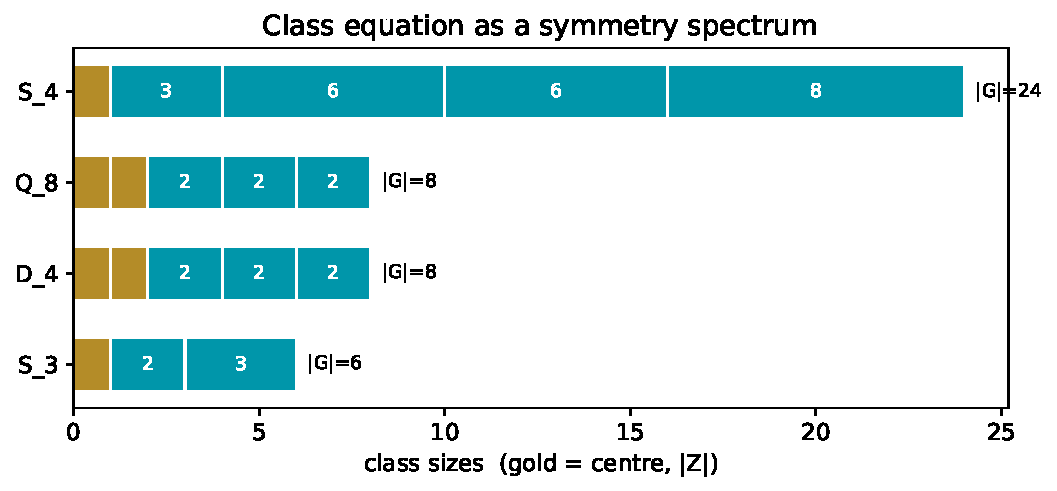
\includegraphics[width=0.84\textwidth]{figures/A2_class_spectrum.pdf}
\caption{The class equation as a symmetry spectrum: conjugacy-class sizes
partition $|G|$ (gold = centre). $D_4$ and $Q_8$ share $8=2+2+2+2$.}
\label{fig:spectrum}
\end{figure}

\noindent\emph{Reading.} A spectrum of many singleton classes (the abelian case,
all gold) means every operation is its own decision cell --- maximal
discrimination. The wide blocks of $S_4$ mean many operations collapse into one
cell. That $D_4$ and $Q_8$ share a spectrum warns that the class equation is a
coarse, though exactly computable, invariant: it bounds the decision granularity
without fully resolving the group.

\subsection{Abelian groups: primary decomposition}

For abelian $G$ the kernel is normal and $\Op=G/L$ factors along its
Sylow-$p$ components.

\begin{theorem}[Primary decomposition]\label{thm:primary}
$G\cong\prod_p G_p$, $L=\prod_p L_p$, and
$\Op\cong\prod_p G_p/L_p=\prod_p\Op_p$.
\end{theorem}

Hence operations factor uniquely into $p$-primary parts, $|\Op|=\prod_p|\Op_p|$,
and a separable cost is optimized componentwise --- a Chinese Remainder
factorization of the decision (Table~\ref{tab:primary}).

\begin{remark}[What it means]
A decision over $\Op$ is equivalent to independent decisions over its
$p$-primary factors. This turns a product-sized search ($\prod_p|\Op_p|$) into a
sum-sized one ($\sum_p|\Op_p|$) --- the operation-level analogue of the discrete
Fourier / CRT speed-up.
\end{remark}

\begin{table}[ht]
\centering
\caption{Primary decomposition of $\Op=C_{12}/\langle 6\rangle$ (computed).}
\label{tab:primary}
\begin{tabular}{lccc}
\toprule
prime $p$ & $|G_p|$ & $|L_p|$ & $|\Op_p|=[G_p:L_p]$ \\
\midrule
$2$ & $4$ & $2$ & $2$ \\
$3$ & $3$ & $1$ & $3$ \\
\midrule
product & $12$ & $2$ & $6=[G:L]$ \\
\bottomrule
\end{tabular}
\end{table}

\noindent\emph{Reading.} The size-$6$ decision space $C_{12}/\langle6\rangle$
\emph{is} $\Op_2\times\Op_3$ ($2\times3$); the kernel itself splits as
$L_2\times L_3$. One never decides over the whole space, only over a
$2$-element and a $3$-element factor.

For a compact connected $G$ the class equation becomes the Weyl integration
formula $\int_G J\,d\mu=\frac{1}{|W|}\int_T J(t)|\Delta(t)|^2dt$. For $SU(2)$ the
class angle carries $(2/\pi)\sin^2\theta\,d\theta$; for $U(n)$ the eigen-phase
density is the squared Vandermonde
\begin{equation}\label{eq:weyl}
d\mu(\theta)=\frac{1}{n!\,(2\pi)^n}\prod_{j<k}\bigl|e^{i\theta_j}-e^{i\theta_k}
\bigr|^2\,d\theta,
\end{equation}
the CUE density, with irreducible characters the Schur polynomials
$\chi_\lambda=s_\lambda(e^{i\theta})$.

\begin{remark}[The validated $SU(2)$ law is the $n=2$ Vandermonde]\label{rem:su2-weyl}
The class density used in \S\ref{sec:apps} is not a separate input: it is \eqref{eq:weyl} at $n=2$. An $SU(2)$
matrix has eigenvalues $e^{\pm i\theta}$, so the squared Vandermonde is
\[
\bigl|e^{i\theta}-e^{-i\theta}\bigr|^2=\bigl|2i\sin\theta\bigr|^2=4\sin^2\theta,
\]
and normalising it to a probability density on the class angle $\theta\in[0,\pi]$ --- where
$\int_0^\pi 4\sin^2\theta\,d\theta=2\pi$ --- gives exactly $\tfrac{2}{\pi}\sin^2\theta$. The repulsion factor
$\sin^2\theta$, i.e.\ eigenvalues avoiding coincidence, is the level repulsion confirmed in
Figure~\ref{fig:weyl}. The finite class equation \eqref{eq:classeq} and the Lie density \eqref{eq:weyl} are thus
one statement --- orbit volume $=$ index$/$stabiliser --- read in the discrete and the continuous regime.
\end{remark}

\section{Applications and comparison with the existing record}
\label{sec:apps}

\subsection{Discrimination of operation spaces}

The generalization turns a large operation space into a few decision cells.
For $S_4$ on $+\bmod 4$ the $12$ twin operations split into $5$ cells of sizes
$\{1,1,2,4,4\}$ under the Weyl group $\Norm_G(L)/L$ of order $2$
(Table~\ref{tab:s4}); the two singletons are the canonical operations.
Figure~\ref{fig:reduction} shows the reduction across several pairs.
\emph{Comparison:} where the prior classification would (incorrectly) read
$\Op$ as a group, the corrected theory reads it as a homogeneous space and
supplies its genuine decision structure.

\begin{table}[ht]
\centering
\caption{Decision data for $S_4$ on $+\bmod 4$ (computed): $L$ non-normal,
$\Op$ a homogeneous space.}
\label{tab:s4}
\begin{tabular}{lc}
\toprule
quantity & value \\
\midrule
$|G|$,\ $|L|$,\ normal? & $24$,\ $2$,\ no \\
$|\Op|=[G:L]$ & $12$ \\
$|\Norm_G(L)|$,\ Weyl $|\Norm_G(L)/L|$ & $4$,\ $2$ \\
decision cells (sizes) & $5$\quad($\{1,1,2,4,4\}$) \\
\bottomrule
\end{tabular}
\end{table}

\begin{figure}[ht]
\centering
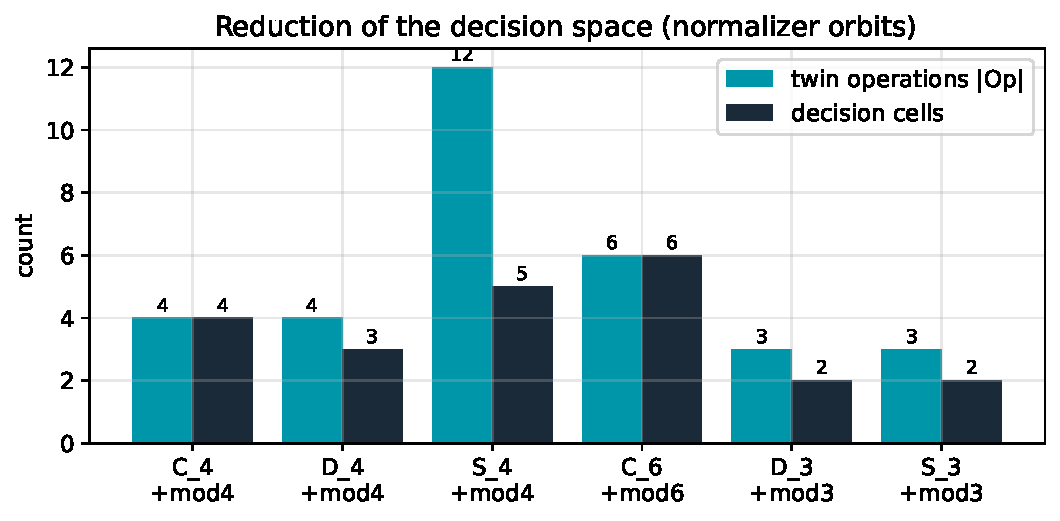
\includegraphics[width=0.84\textwidth]{figures/A1_reduction.pdf}
\caption{Reduction of the decision space: distinct twin operations $|\Op|=[G:L]$
vs decision cells (orbits of $\Norm_G(L)$), for finite $(G,+\bmod m)$ pairs.}
\label{fig:reduction}
\end{figure}

\noindent\emph{Reading.} The gap between the two bars is the dividend of the
theory: for $S_4$ a $12$-way choice becomes a $5$-way one. The gap is widest for
the richest non-abelian groups, where conjugation identifies the most
operations.

\subsection{The Weyl measure against random-matrix statistics}

The Lie generalization is validated against the existing spectral record. The
$SU(2)$ class density matches $(2/\pi)\sin^2\theta$
(Figure~\ref{fig:weyl}, left); the CUE moments $\mathbb{E}[\mathrm{tr}\,U]=0$,
$\mathbb{E}|\mathrm{tr}\,U|^2=1$ are recovered for $U(2),U(3),U(4)$
(Figure~\ref{fig:weyl}, right; Table~\ref{tab:cue}); and the measure
\eqref{eq:weyl} is pinned down by Schur-character orthonormality
$\langle\chi_\lambda,\chi_\mu\rangle=\delta_{\lambda\mu}$
(Figure~\ref{fig:orth}). \emph{Comparison:} these reproduce classical
random-matrix and representation-theoretic facts \cite{mehta,fulton}, confirming
that the decision measure on qudit gate classes is the correct one.

\begin{table}[ht]
\centering
\caption{CUE moments under the Weyl measure (Haar Monte-Carlo, $2{\times}10^4$
samples).}
\label{tab:cue}
\begin{tabular}{lccc}
\toprule
 & $U(2)$ & $U(3)$ & $U(4)$ \\
\midrule
$\mathbb{E}[\mathrm{tr}\,U]$ (target $0$) & $\approx 0.00$ & $\approx 0.00$ & $\approx 0.01$ \\
$\mathbb{E}|\mathrm{tr}\,U|^2$ (target $1$) & $1.01$ & $0.99$ & $1.00$ \\
\bottomrule
\end{tabular}
\end{table}

\begin{figure}[ht]
\centering
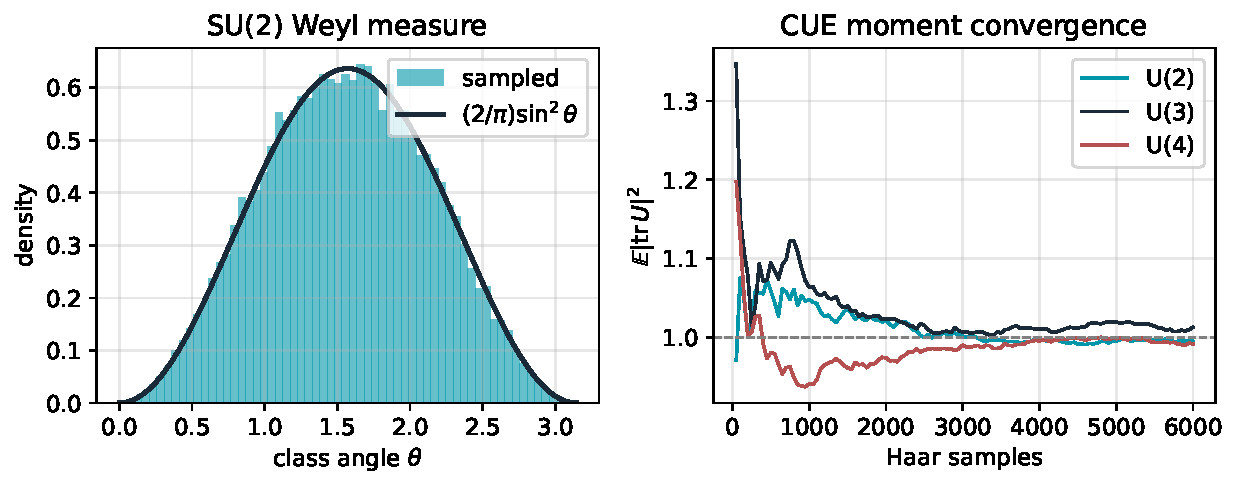
\includegraphics[width=0.96\textwidth]{figures/A3_weyl.pdf}
\caption{Left: $SU(2)$ class-angle density, sampled vs $(2/\pi)\sin^2\theta$.
Right: convergence of $\mathbb{E}|\mathrm{tr}\,U|^2\to 1$ for $U(2),U(3),U(4)$.}
\label{fig:weyl}
\end{figure}

\noindent\emph{Reading.} The left panel is a direct, visual confirmation that
our class measure on $SU(2)$ is the Weyl law, not an artefact; the right panel
shows the same for higher rank through a moment that the measure must return as
exactly $1$. Agreement here is what licenses decisions taken against
\eqref{eq:weyl}.

\begin{figure}[ht]
\centering
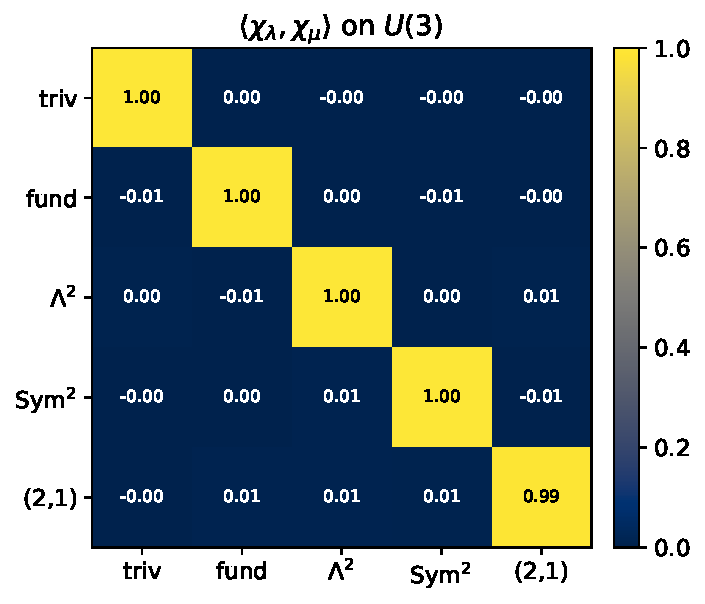
\includegraphics[width=0.48\textwidth]{figures/A4_orthonormality.pdf}
\caption{Computed Gram matrix $\langle\chi_\lambda,\chi_\mu\rangle$ of Schur
characters on $U(3)$: the identity, confirming the Weyl measure \eqref{eq:weyl}.}
\label{fig:orth}
\end{figure}

\noindent\emph{Reading.} Orthonormality is the sharpest possible check: the
characters form an orthonormal basis of class functions \emph{only} under the
correct measure, so a Gram matrix indistinguishable from the identity pins down
\eqref{eq:weyl} uniquely. The off-diagonal noise ($\sim10^{-2}$) is the
Monte-Carlo error, not a systematic deviation.

\subsection{Classical magma counts as special cases}

Finally, the orbit machinery reproduces the existing enumeration of
$G$-invariant magmas, $\prod_O|\mathrm{Fix}_E(\mathrm{Stab}_G(O))|$: the cyclic
count $C_n\mapsto n^n$, the symmetric collapse $S_n\,(n\ge 4)\mapsto 2$, and the
linear-group stabilization $\mathrm{GL}_n(\mathbb{F}_q)\mapsto q^{q+3}$ (computed
for small cases). \emph{Comparison:} these classical counts emerge as a
by-product of the same decision-cell decomposition. Table~\ref{tab:compare}
summarizes the arc.

\begin{table}[ht]
\centering
\caption{The four-movement arc: antecedents, their place, their generalization,
and the new outcome.}
\label{tab:compare}
\begin{tabular}{p{3.1cm}p{2.7cm}p{3.0cm}p{4.0cm}}
\toprule
antecedent & as twin ($G$) & generalizes to & new outcome \\
\midrule
multiplicative calculus \cite{grossman} & $\langle\log\rangle$ &
arbitrary $G$ & class-equation discrimination \\
exponential hierarchy & $\langle\exp\rangle\cong\Z$ &
finite / abelian / Lie & corrected classification (homog.\ space) \\
CUE eigenvalue statistics \cite{mehta} & conjugation by $U(n)$ &
qudit class costs & Weyl-verified decision measure \\
invariant-magma counts & finite $G$ on $E^2$ &
normalizer orbits & decision-cell reduction \\
\bottomrule
\end{tabular}
\end{table}

\noindent\emph{Reading.} Read left to right, each row is the arc in miniature: a
known construction, its home in the general theory, the direction it
generalizes, and the new result that follows. The framework's value is that the
same final column is produced by one machine for every row.

All results are realized in \code{arithmetics.symbolic.twin} (SymPy, NumPy,
mpmath): exact finite-group computation (conjugacy, centralizers, centre,
normality, quotients), exact one-parameter analysis for $SU(2),SO(2)$, Haar
Monte-Carlo for $SO(3),SU(n)$, and Schur characters by the bialternant. The
figures and tables are regenerated by \code{papers/make\_figures.py}; each
theorem is paired with a unit test ($131$ tests pass).

\section{Discussion}

The arc closes a gap: classical generator-function arithmetics are unified as
twin operations, generalized from $\Z$ to arbitrary symmetry, and discriminated
by a single family of invariants that simultaneously recovers known counts,
matches random-matrix statistics, and corrects a normality error. The honest
limitation is structural: by equivariance every twin operation is isomorphic to
the base, so the discriminating invariants are conjugation-level (the class
equation) or frame-dependent --- the latter is the subject of the companion,
technological paper.

\appendix

\section{Complete proofs}
\label{app:proofs}

\paragraph{Theorem~\ref{thm:orbits} (normalizer orbits).}
We first show the relabeling $r_w:\odot_{eg}\mapsto\odot_{e,wgw^{-1}}$ is
well defined on $\Op$ iff $w\in\Norm_G(L)$. By Proposition~\ref{prop:fibres}
$\odot_{eg}$ determines, and is determined by, the right coset $Lg$. For $a\in L$,
$w(ag)w^{-1}=(waw^{-1})(wgw^{-1})$, so $L\,w(ag)w^{-1}=L\,wgw^{-1}$ for all $a\in
L$ iff $waw^{-1}\in L$ for all $a\in L$, i.e. iff $wLw^{-1}=L$. Hence $r_w$ is a
well-defined map $\Op\to\Op$ exactly for $w\in\Norm_G(L)$, and
$w\mapsto r_w$ is a group action of $\Norm_G(L)$ (since $r_w r_{w'}=r_{ww'}$ on
cosets). The decision cells are its orbits; by Burnside their number is
$\frac{1}{|\Norm_G(L)|}\sum_{w}|\mathrm{Fix}(r_w)|$. If $L\trianglelefteq G$ then
$\Norm_G(L)=G$ and $r_w$ is conjugation on $G/L$, whose orbits are the conjugacy
classes. $\qed$

\paragraph{Theorem~\ref{thm:primary} (primary decomposition).}
Let $|G|=\prod_i p_i^{a_i}$ and $G_p=\{g:\mathrm{ord}(g)=p^k\}$. For each $p$ put
$q=|G|/p^{a}$ and choose, by B\'ezout, $u$ with $uq\equiv 1\ (\mathrm{mod}\
p^{a})$; set $e_p=uq$, so $e_p\equiv 1\ (\mathrm{mod}\ p^{a})$ and
$e_p\equiv 0\ (\mathrm{mod}\ p'^{a'})$ for $p'\neq p$. Then
$\pi_p(g):=g^{e_p}\in G_p$ and $\sum_p e_p\equiv 1\ (\mathrm{mod}\ |G|)$, whence
$\prod_p\pi_p(g)=g$; this realises $G\cong\prod_p G_p$. Any subgroup $L\le G$ is a
finite abelian group, so $L=\prod_p(L\cap G_p)=\prod_p L_p$. Quotienting
factorwise gives $G/L\cong\prod_p G_p/L_p$. $\qed$

\paragraph{Proposition~\ref{prop:classfn} (class-function reduction).}
If $J$ is a class function and $x,x'$ are conjugate, $J(x)=J(x')$; thus $J$ is
constant on each conjugacy class and $\arg\min J$, being defined by a value of
$J$, is a union of classes. Evaluating one representative per class therefore
suffices, and \eqref{eq:classeq} counts the classes with multiplicities. $\qed$

\paragraph{Counting formula.}
A $G$-invariant magma is a $G$-equivariant map $\odot:E\times E\to E$. Equivariance
fixes $\odot$ on a whole orbit $O\subseteq E\times E$ once its value at a
representative $(i,j)$ is chosen; that value must lie in
$\mathrm{Fix}_E(\mathrm{Stab}_G(i,j))$. Independent choices over orbits give
$\prod_O|\mathrm{Fix}_E(\mathrm{Stab}_G(O))|$. $\qed$

\section{Worked computation: \texorpdfstring{$S_4$ on $+\bmod 4$}{S4 on +mod4}}
\label{app:s4}

The structural kernel is $L=\{e,(1\,3)\}$, of order $2$. Its normalizer is
$\Norm_{S_4}(L)=\{e,(1\,3),(0\,2),(0\,2)(1\,3)\}$ of order $4$ (the centraliser
of the involution $(1\,3)$), so the Weyl group $\Norm_G(L)/L$ has order $2$,
generated by the image of $(0\,2)$. The conjugacy classes of $S_4$ have sizes
$1,6,3,8,6$ (identity, transpositions, double transpositions, $3$-cycles,
$4$-cycles). The $\Norm_G(L)$-action on the $[G:L]=12$ operations has the orbit
profile $\{1,1,2,4,4\}$: two fixed operations (the canonical, robust choices),
one $2$-orbit, and two $4$-orbits. A purely structural criterion thus reduces
the $12$-way choice to $5$ cells, ranked by symmetry.

\section{Finite discovery table}
\label{app:disc}

Table~\ref{tab:disc-full} lists the computed classification across a catalogue of
finite groups and two base operations ($+\bmod m$ and the rigid left projection
$x\odot y=x$). The left projection is preserved by every permutation ($L=G$,
one cell); the additions are non-trivial, and $L$ is non-normal exactly for the
non-abelian groups, where $|\Op|=[G:L]$ exceeds the cell count.

\begin{table}[ht]
\centering
\caption{Computed twin-operation classification (decision cells via
$\Norm_G(L)$-orbits).}
\label{tab:disc-full}
\begin{tabular}{llccccc}
\toprule
Group & base & $|G|$ & $|L|$ & $[G:L]$ & $L\trianglelefteq G$ & cells \\
\midrule
$C_2$ & $+\bmod 2$ & 2 & 1 & 2 & yes & 2 \\
$C_3$ & $+\bmod 3$ & 3 & 1 & 3 & yes & 3 \\
$C_4$ & $+\bmod 4$ & 4 & 1 & 4 & yes & 4 \\
$V_4$ & $+\bmod 4$ & 4 & 1 & 4 & yes & 4 \\
$D_3$ & $+\bmod 3$ & 6 & 2 & 3 & no  & 2 \\
$D_4$ & $+\bmod 4$ & 8 & 2 & 4 & no  & 3 \\
$S_3$ & $+\bmod 3$ & 6 & 2 & 3 & no  & 2 \\
$S_4$ & $+\bmod 4$ & 24 & 2 & 12 & no & 5 \\
\midrule
any  & left-proj  & $|G|$ & $|G|$ & 1 & yes & 1 \\
\bottomrule
\end{tabular}
\end{table}

\noindent\emph{Reading.} The table separates three regimes at a glance:
\emph{rigid} (left projection, one cell, $L=G$); \emph{abelian non-trivial}
($L$ trivial and normal, $\Op$ a group of size $[G:L]$); and \emph{non-abelian}
($L$ non-normal, so $\Op$ is only a homogeneous space and the cell count drops
below $[G:L]$). The last regime is exactly where the correction of
Remark~\ref{rem:correction} bites.

\begin{thebibliography}{9}
\bibitem{grossman} M.~Grossman, R.~Katz, \emph{Non-Newtonian Calculus},
Lee Press, 1972.
\bibitem{gerstenhaber} M.~Gerstenhaber, On the deformation of rings and
algebras, \emph{Ann.\ of Math.} 79 (1964), 59--103.
\bibitem{weyl} H.~Weyl, \emph{The Classical Groups}, Princeton Univ.\ Press, 1939.
\bibitem{mehta} M.~L.~Mehta, \emph{Random Matrices}, 3rd ed., Elsevier, 2004.
\bibitem{mezzadri} F.~Mezzadri, How to generate random matrices from the
classical compact groups, \emph{Notices AMS} 54 (2007), 592--604.
\bibitem{fulton} W.~Fulton, J.~Harris, \emph{Representation Theory}, Springer, 1991.
\end{thebibliography}

\end{document}
